\documentclass{ximera}

\author{Anna Davis} \title{MTH 140 Homework 3} 

\begin{document}

\begin{abstract}

\end{abstract}
\maketitle
 \textit{Certificate due: 2/1/2021 at 11:59 p.m.}
 
 \begin{problem}\label{prob:140hom2prob3}
The histogram below shows the number of absences that occurred over one semester period in Mrs. Miller's fifth grade class.  For example, this graph tells us that the number of students incurring 2 absences is 5.

\begin{image}
   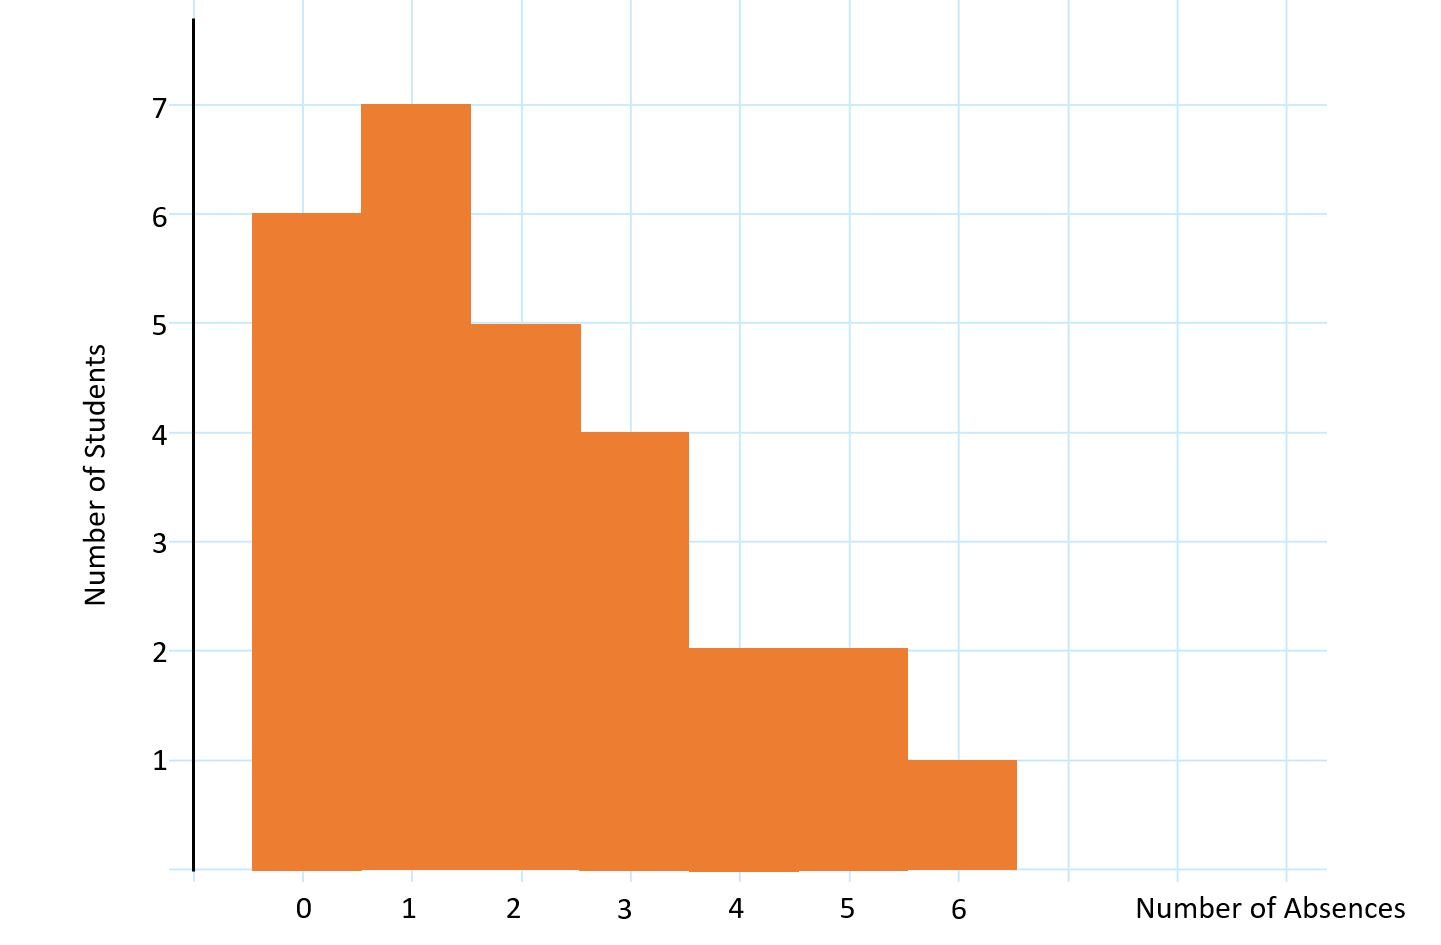
\includegraphics[height=1in]{140H2pic6.jpg}
 \end{image}
 
 Use the graph to answer the following questions.
 
 \begin{enumerate}
     \item How many students incurred 3 absences? $\answer{4}$
     \item What is the mode? $\answer{1}$
     \item How many students are in the class? $\answer{27}$
     \item What is the mean number of absences? $\answer[tolerance=0.01]{1.96}$
     \item What is the median number of absences? $\answer{2}$
 \end{enumerate}
\end{problem}

\begin{problem}\label{prob:140hom2prob4}
The following is a summary of test results for an introductory History course.
\begin{image}
   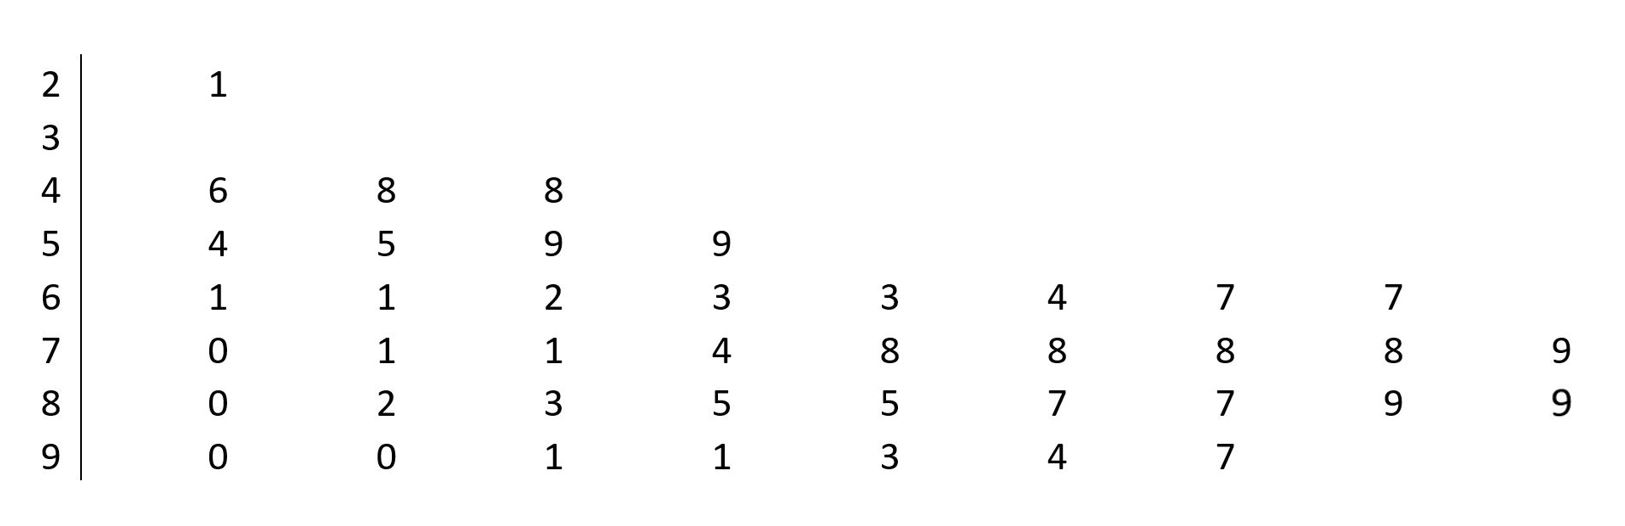
\includegraphics[height=1in]{140H2pic10.jpg}
 \end{image}
 
 Use this information to answer the following questions.
 
 \begin{enumerate}
     \item How many students took the test? $\answer{41}$
     \item What is the mode? $\answer{78}$
     \item What is the median score? $\answer{78}$
     \item $Q1=\answer{61.5}$
     \item $Q3=\answer{87}$
     \item $\mbox{IQR}=\answer{25.5}$
     \item Outlier Score(s): $\answer{21}$
     \item 20 th percentile is $\answer{60}$
     \item 60 th percentile is $\answer{79.5}$
     \item 80 th percentile is $\answer{89}$
 \end{enumerate}
\end{problem}

\begin{problem}\label{prob:140hom2prob5}
A perfectly good box plot was damaged by a coffee spill.  
\begin{image}
   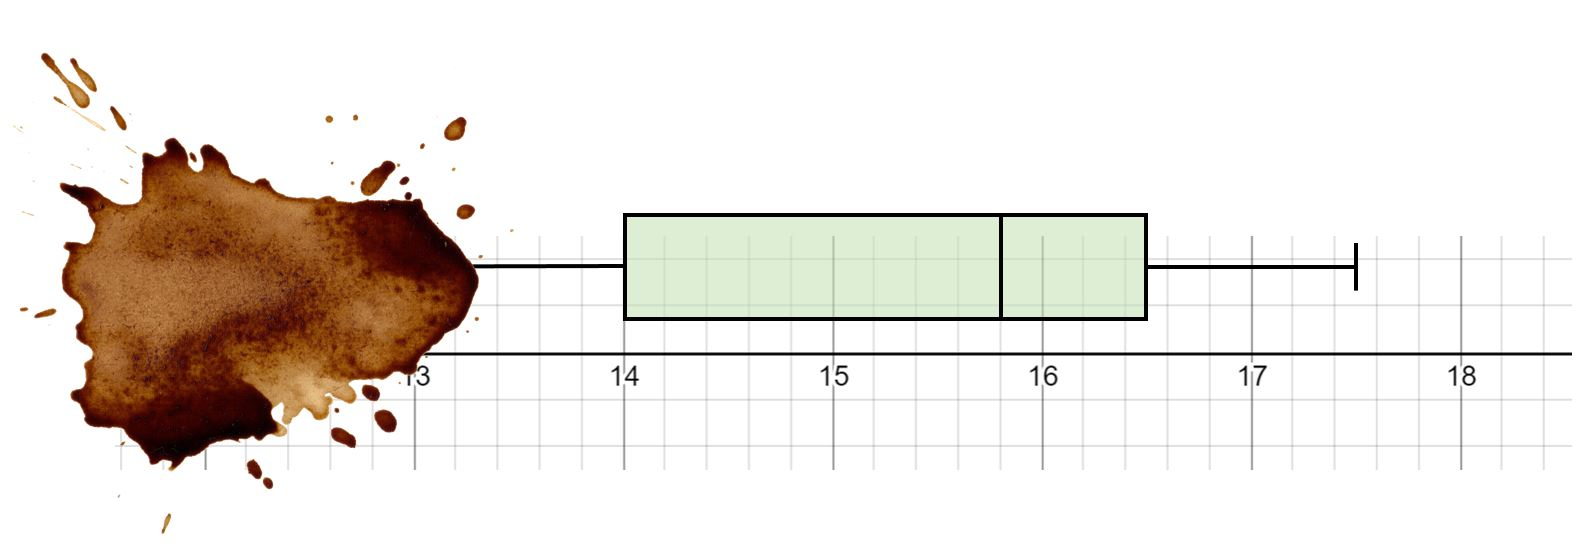
\includegraphics[height=1in]{140H2pic9.jpg}
 \end{image}
 Try to answer each of the following questions.
 \begin{enumerate}
     \item The largest value in the data set is 
     \wordChoice{\choice[correct]{$17.5$}, \choice{$16.5$},\choice{Cannot be determined}}
     \item The smallest value in the data set is 
     \wordChoice{\choice{$10$}, \choice{$14$},\choice[correct]{Cannot be determined}}
     \item $\mbox{IQR}=\answer{2.5}$
     \item Is 10 an outlier? 
     \wordChoice{\choice[correct]{Yes}, \choice{No},\choice{Cannot be determined}}
 \end{enumerate}
 
 \end{problem}
 
 
 
 
 
 
 
 
\begin{problem}\label{prob:140hom3prob1}

Use the table below to compute sample standard deviation ($s$), for the following SAMPLE of test scores:
$$68, 73, 75, 81, 94$$

$$n=\answer{5}$$
$$\overline{x}=\answer{78.2}$$
Enter EXACT values into the table; no rounding.
\begin{center}
\begin{tabular}{|c|c|c|}
Test Scores & Deviations & Deviations Squared  \\
 \hline
 \hline
   & &\\
 68 &$\answer{-10.2}$  & $\answer{104.04}$ \\
  & &\\
  \hline
   & &\\
 73 &$\answer{-5.2}$  & $\answer{27.04}$\\
  & &\\
 \hline
  & &\\
 75 &$\answer{-3.2}$ &$\answer{10.24}$ \\
  & &\\
 \hline
  & &\\
 81 &$\answer{2.8}$  &$\answer{7.84}$ \\
  & &\\
 \hline
  & &\\
 94 &$\answer{15.8}$  &$\answer{249.64}$ \\
  & &\\
 \hline
  
\end{tabular}
\end{center}

$$s =\sqrt{\frac{\sum (x-\overline{x})^2}{n-1}}=\answer[tolerance=0.1]{10}$$
 \end{problem}


\begin{problem}\label{prob:140hom3prob2}
There are four gas stations in a small town.  One day in July, the gas prices were as follows:
$$1.94, 1.94, 1.99, 2.01$$
Fill out the table below to find the population standard deviation ($\sigma$).
$$N=\answer{4}$$
$$\mu=\answer{1.97}$$
Enter EXACT values into the table; no rounding.
\begin{center}
\begin{tabular}{|c|c|c|}
Price per Gallon & Deviations & Deviations Squared  \\
 \hline
 \hline
   & &\\
 1.94 &$\answer{-0.03}$  & $\answer{0.0009}$ \\
  & &\\
  \hline
   & &\\
 1.94 &$\answer{-0.03}$  & $\answer{0.0009}$\\
  & &\\
 \hline
  & &\\
 1.99 &$\answer{0.02}$ &$\answer{0.0004}$ \\
  & &\\
 \hline
  & &\\
 2.01 &$\answer{0.04}$  &$\answer{0.0016}$ \\
  & &\\
 \hline
 
\end{tabular}
\end{center}
Round $\sigma$ to four decimal places.
$$\sigma =\sqrt{\frac{\sum (x-\mu)^2}{N}}=\answer[tolerance=0.0001]{0.0308}$$
\end{problem}


\end{document} 


